\documentclass[../ProgettoTecWeb2.tex]{subfiles}

\begin{document}
\section{Considerazioni generali sul sito}
	
	\subsection{Link}
	Nel sito web non si riscontra l'utilizzo di colori differenti per i link visitati e per i link non ancora visitati. Tale scelta, combinata al non utilizzo dei breadcrumbs in tutte le pagine, può dare vita al problema del \textit{Lost in navigation}: un utente, durante la navigazione, non sa più dove si trova nella gerarchia del sito web, perde tempo e si arrabbia. Non colorando i collegamenti ipertestuali, inoltre, si richiede all'utente uno sforzo computazionale per ricordare le pagine visitate. Inoltre, nel web, è sempre meglio attenersi alle convenzioni e quindi colorare i link di colori differenti. Inoltre alcuni link vengono sottolineati quando ci si passa sopra col mouse, altri no: sarebbe preferibile mantenere sempre la stessa visualizzazione (e forse sottolineari tutti in modo tale da evidenziare il fatto che sono link).

		\subsubsection{404}
		Provando ad accedere ad una pagina inesistente oppure non più disponibile il sistema provvede a caricare una pagina che spiega questo errore. Tale scelta è la migliore possibile per questo tipo di situazioni. Per di più la pagina visualizzata utilizza l'ironia (in tema videogames) per spiegare l'errore e ciò è molto apprezzato dagli utenti.
		\begin{figure} [H]
			\centering
			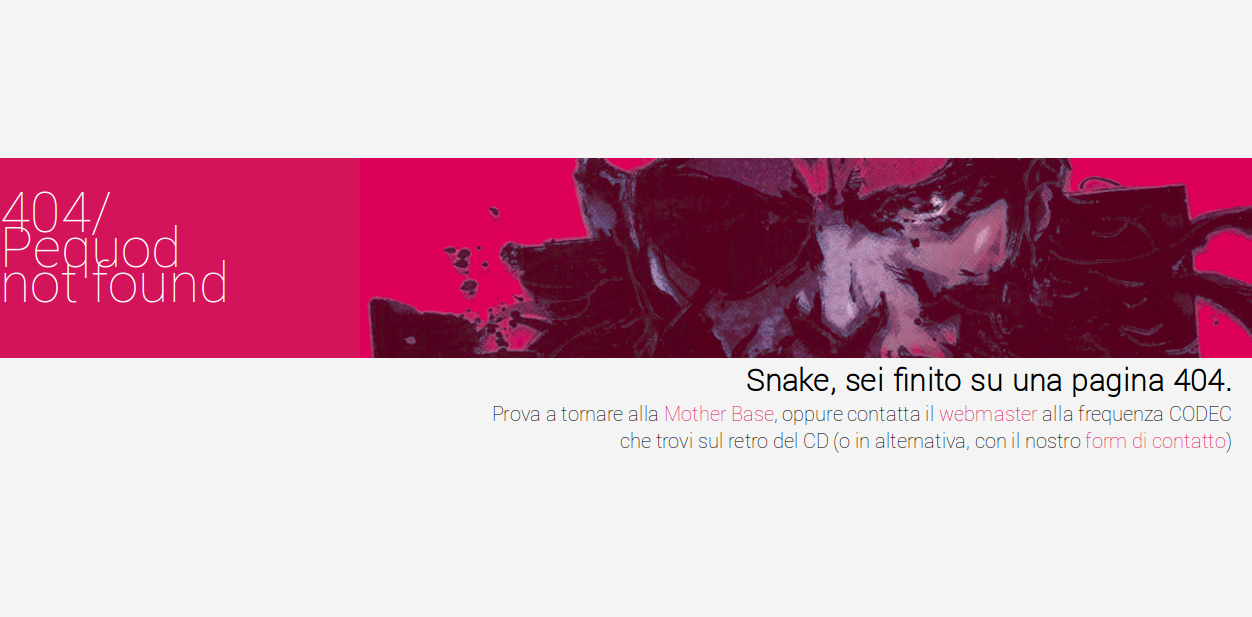
\includegraphics[scale=0.3]{img/404}
			\caption{Pagina 404}
		\end{figure}

	\subsection{Apertura nuove finestre e pop-up}
	Aprendo i vari link presenti nel sito non sono state registrate aperture di nuove finestre e pop-up. Ciò è positivo e permette una navigazione non dispersiva.

	\subsection{Back button}
	Non si registrano modifiche al comportamento del tasto back del browser. Questo è facilitato dall'utilizza sempre della stessa finestra di navigazione ed è apprezzato dagli utenti poichè abituati all'utilizzo del back button.

	\subsection{Testo}
	Il testo contenuto nel sito presenta in generale una buona dimensione ed un buon grado di contrasto rispetto allo sfondo: il testo normale è di colore nero su sfondo bianco oppure grigio chiaro, mentre link e titoli sono di colore blu o rosa scuro, sempre sugli stessi colori di sfondo. Da registrare un minor contrasto tra lo sfondo del menù e le voci dello stesso. Le voci non selezionate sono di colore bianco e lo sfondo è grigio. Il sito non offre opzioni per il resize del testo e quindi, per questo, bisogna affidarsi al browser. Non vengono utilizzati molti effetti nel testo. Viene utilizzato solamente il grassetto per evidenziarne alcune parti. Il font utilizzato è il Verdana (il preferito dagli utenti del web). \\
	
	Il testo è solitamente diviso in blocchi, ogniuno dei quali contenente un titolo (di solito non troppo lungo). Non sono spesso utilizzati liste o elenchi, anche se aiutano la memorizzazione di quanto letto, e le parti di testo evidenziate a volte sono troppo grandi. \\
	
	Spesso il testo presentato è veramente molto lungo. Non è prevista la possibilità di cambiare lingua di fruizione del sito.

	\subsection{Scoll}
	In generale nel sito le pagine superano di molto la grandezza consigliata costringendo l'utente ad effettuare molto scroll verticale. Questo problema è accentuato dalla scelta di presentare alcune pagine come una griglia ``infinita'' dei contenuti. Non è prevenuto invece scroll orizzontale poichè le pagine si adattano alla larghezza della finestra di navigazione.

	\subsection{Design}
	Il design del sito si presenta abbastanza chiaro e pulito. Non sono stati trovati elementi che possano essere assimilabili a bloated design, metafore visive o metafore metafisiche. Sono spesso presenti video nelle pagine interne: a mio giudizio completano i contenuti e la loro presenza è positiva.
\end{document}
